\begin{figure}
    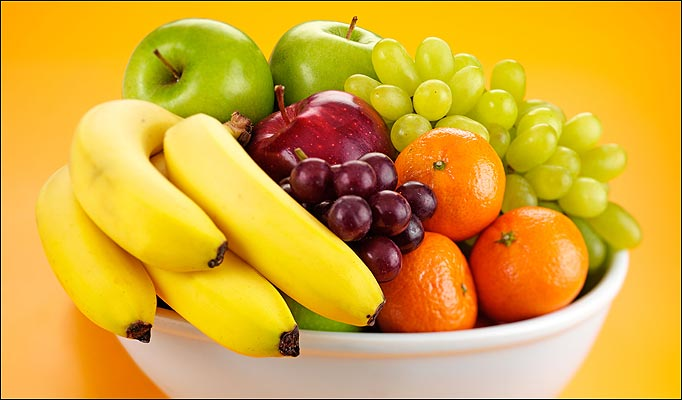
\includegraphics[scale=0.5]{fruitbowl2}
    \caption{Alternative Bowl of fruit}
    \label{fig:newFruit}
\end{figure}

\begin{table}[]
    \centering
    \caption{Comparison of fruit bowl images}
    \label{newFruitTable}
    \begin{tabular}{lllllll}
        Food type & Grid & Row & Column & New Grid & New Row & New Column \\
        Apple     & 5    & 1   & 3      & 4        & 1       & 0          \\
        Banana    & 1    & 0   & 1      & 5        & 0       & 5          \\
        Grape     & 4    & 0   & 0      & 2        & 1       & 0          \\
        Orange    & 5    & 0   & 0      & 0        & 0       & 0          \\
        Other     & 0    & 3   & 1      & 1        & 2       & 1         
    \end{tabular}
\end{table}

\subsection*{Overview}
In our three previous sliding window oriented experiments, we had only used a
single image. In order to see whether this image had biases unknown
to us, I decided to use another fruit bowl image. This image was selected as
fruit took up a larger portion of the image as seen in Figure \ref{fig:newFruit}

\subsection*{Results}
\subsubsection*{Grid}
The performance of this experiment was slightly worse than with the previously
used image. When I ran the grid based sliding window on Figure
\ref{fig:newFruit}, fourteen out of fifteen predictions had an expected value.
Out of the fourteen predictions orange was not predicted to top-1 accuracy at
all. This can be seen, in comparision to previously used image, in Table
\ref{newFruitTable}.

\subsubsection*{Row}
In the column based window for the new fruit image, the results were not very
successful as has been the trend for most row based classification. Two out of
four predictions had an expected value at top-1 accuracy.

\subsubsection*{Column}
The column based approach had a similar result to its counterpart in that only
one of its predictions was unexpected. Although, due  to the size of the new
image, another column was created and thus has a better overall accuracy.

\subsection*{Empirical Analysis}
A possible reason that an orange was not classified in any of these images is
because in Figure \ref{fig:newFruit}, a more mandarin food is displayed.
